%Vorbereitung: Baendermodell, generation und rekombination von ladungstraegern, Intensitaetsabhaengigkeit der photoleitfaehigkeit, frequenzabhaengigkeit der photoleitfaehigkeit

\subsection{Theoretischer Hintergrund}
\subsubsection{Bändermodell}
Die quantenmechanischen Energiezustände in einem Kristall lassen sich mit dem so genannten Bändermodell beschreiben.
In einem konstanten Potential lassen sich Elektronen mit ebenen Wellen mit quadratischer Dispersionsrelation beschreiben. 
Im periodischen Potential der im Gitter angeordneten Atomrümpfe interferieren die ebenen Wellen mit den am Potential gestreuten.
Am Rande der Brioullin Zonen entsteht konstruktive Interferenz und es entstehen stehende Wellen. Für stehende Wellen gibt es zwei phasenverschobene Lösungen mit gleicher kinetischer Energie. Die Gesamtenergie ist für die beiden Lösungen unterschiedlich aufgrund von unterschiedlichen Aufenthaltswahrscheinlichkeiten im hohen bzw. niedrigen Potential.
An den Rändern der Brillouin Zonen kommt es also zu Energiebereichen, in denen es keine Lösungen für die Wellenfunktion gibt.\\
Außerdem ist die Gruppengeschwindigkeit einer stehenden Welle:
$$v \propto \frac{\partial E}{\partial k_x} = 0$$
die Steigung geht also am Zonenrand gegen $0$ und es entsteht das bekannte Bandzonenschema.


\subsubsection{Fermi-Statistik}
Als Spin-1/2-Teilchen folgen Elektronen der Fermi-Dirac Verteilung. Sie misst die Besetzungswahrscheinlichkeit eines Zustandes und ist gegebe durch:
$$f_{FD} = \frac{1}{\mathrm{exp}(\frac{E-E_F}{k_B T})+1} $$
Hierbei ist E die Energie des Zustandes, $k_B$ die Boltzmann-Konstante und $E_F$ die Fermi-Energie, bei der die Besetzungswahrscheinlichkeit 1/2 ist. \\
Bei Halbleitern liegt die Fermi-Energie typischerweise zwischen dem Leitungs- und dem Valenzband. Ist der Abstand der Fermi-Energie zu beiden Bandkanten groß im Vergleich zur thermischen Energie $k_B T$, so kann sie durch die Boltzmann Verteilung angenähert werden:
$$f_{B} = e^{-(E-E_F) / k_B T}$$
Halbleiter, für die diese Näherung zutrifft nennt man nicht entartete Halbleiter.

\newpage

\subsubsection{Dotierung}
Dotierung eines Halbleiters ist die gezielte Verunreinigung durch bestimmte Atome. Abhängig von diesen Atomen spricht man von p- und n-Dotierung. Nehmen sie die Rolle eines Donators ein, geben also ein Elektron ab in das Leitungsband, da die Energielücke zwischen Donatorniveau und Leitungsband sehr klein ist, so handelt es sich um n-Dotierung. Umgekehrt nehmen Akzeptoren Elektronen aus dem Valenzband leicht auf, da ihr Energieniveau nahe an diesem liegt und so ein Defektelektron entsteht. \\
Auf diese Weise gibt es eine bestimmte Art Majoritätsladungsträger, nämlich entweder Elektronen oder Löcher. \\
Im thermischen Gleichgewicht gilt mit dem Index i für intrinsisch:
$$ n \cdot p = n_i^{2} (T) $$
Hierbei ist zu beachten, dass $n_i$ zunächst eine reine Rechengröße ist, für hohe Energien jedoch $n = p$ gilt und sie somit die Ladungsträgerdichte beschreibt. \\
Für niedrige Energien ist die Leitfähigkeit jedoch vollständig von den Majoritätsladungsträgern bestimmt, da erst für hohe Temperaturen Elektron-Loch-Paare aus dem ursprünglichen Halbleiter beitragen. Abb. 1.1 zeigt die Ladungsträgerkonzentration über der Temperatur für n-dotiertes Germanium.
\begin{figure}
\centering
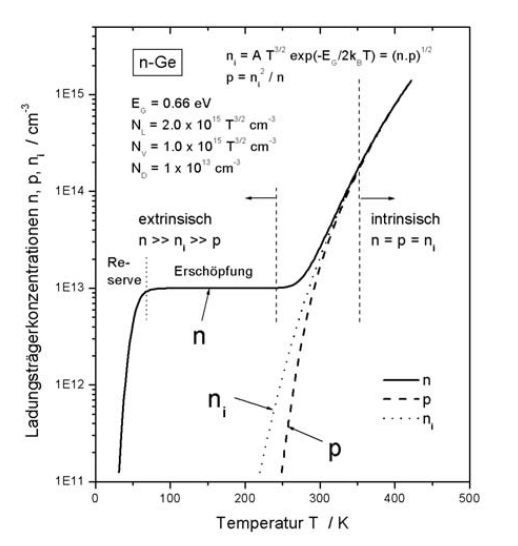
\includegraphics[scale=0.5]{./chap/Ladungstrkonz_temp.png}[b]
\caption{Ladungsträgerkonzentration über der Temperatur für n-dotiertes Gallium. Entnommen aus der Vorbereitungsmappe.}
\end{figure}
Im Bereich 'Reserve' werden die Majoritätsladungsträger durch die Dotierung bestimmt leitfähig, im Bereich 'Erschöpfung' sind alle leitfähig, jedoch noch keine Elektron-Loch-Paare von Germanium selbst. Letztere überwiegen im intrinsischen Bereich.
\subsubsection{Ladungsträgerbeweglichkeit}
Die Ladungsträgerbeweglichkeit ist lediglich beschränkt durch Störungen eines perfekten Gitters. Im Folgenden sind einige aufgelistet.\\
\paragraph{Geladene Störstellen} streuen mittels herkömmlicher Rutherfordstreuung. Mit $v \propto \sqrt{T}$ im thermischen Gleichgewicht folgt:
$$\mu \propto T^{3/2} $$
\paragraph{Akustische Phononen} streuen nicht-polar und polar. Die Beweglichkeit folgt hierbei:
$$\mu _{3D} \propto T^{-3/2} $$
$$\mu _{2D} \propto T^{-1} $$
\paragraph{Optische Phononen} streuen auch nicht-polar, sowie polar. Die Temperaturabhängigkeit ist im 2D- und 3D-Fall gegeben durch die Bose-Einstein-Verteilung:
$$\mu \propto e^{\frac{\hbar \omega}{k_B T}} -1 $$
\paragraph{Zwischentalstreuung} tritt auf wegen Streuung an den Energieminima der Bandstruktur. Nennenswert ist dieser Effekt erst ab 100K.
\paragraph{Elektron-Loch-Streuung} ist relevant bei hohen Temperaturen, bzw. im intrinischen Bereich.\\
\newline
Da die Streuraten sich addieren, addieren sich die Kehrwerte der Beweglichkeit.

\subsubsection{2D Elektronengas}
Ein 2 dimensionales Elektronengas kann an einer Grenzschicht zwischen einem n-dotierten und reinen Halbleiter näherungsweise erzeugt werden.\\
An der Kontaktschicht diffundieren Elektronen des dotierten Halbleiters in das Leitungsband des reinen Halbleiters. Diese werden durch die Donatoren an der Grenzschicht gehalten, können aber die vorhandene Bandkante nicht überqueren. Die Elektronendichte ist dort hoch, da sie unterhalb der Fermienergie sind. Außerdem sind sie räumlich getrennt von ihren Donatoren und bilden ein 2 dimensionales Elektronengas, da sie sich nur noch in einer Ebene bewegen können.\\
Auf Grund der räumlichen Trennung von Elektronen und Donatoren können hohe Beweglichkeiten erreicht werden, da keine Störstellenstreuung auftritt.
\subsubsection{Leitfähigkeit}
Die Stromdichte ist gegeben durch 
$$J = \rho \cdot \nu _d = - e n \cdot \nu _d$$
mit der Driftgeschwindigkeit $\nu _d$, der durch das elektrische Feld erzeugten Geschwindigkeit der Elektronen und der Elektronendichte $n$. Weiterhin gilt folgende Gleichung:
$$\nu _d = - \frac{e \tau}{m} E =: -\mu E $$
Hierbei ist $\mu$ die Elektronenbeweglichkeit und $\tau$ die Stoßzeit zweier Elektronen. Die erste Gleichheit stammt aus dem Ansatz von Drude im stationären Fall, die zweite Gleichheit ist die Definition der Elektronenbeweglichkeit. \\
Zusammen mit dem Ohmschen Gesetz folgt für die Leitfähigkeit
$$\sigma = en\mu $$
\subsubsection{Halleffekt}
Der Halleffekt beschreibt die Ablenkung eines Stromes in einem von einem B-Feld durchsetzen Material. Hierbei werden die Elektronen durch die Lorentzkraft abgelenkt, wodurch im Gleichgewicht eine Spannung senkrecht zur Stromrichtung und Richtung des B-Feldes abgegriffen werden kann. Hierfür gilt:
$$E_H = -R_H \cdot (J \times B) $$
Mit der Hallkonstanten $R_H = \frac{1}{nq}$ und der Stromdichte $J$.\\
Treten nicht nur Elektronen sondern auch Löcher als Ladungsträger auf, so spricht man von bipolarer Leitung im Gegesatz zu obiger unipolarer Leitung. Die Löcher werden in die gleiche Richtung abgelenkt und für die Hallkonstante folgt mit $b = \frac{\mu _n}{\mu _p}$:
$$R_H^{bip} = \frac{1}{\vert e \vert \cdot n_i} \cdot \frac{1 - b}{1 + b}$$
Im extrinsischen Bereich eines n-dotierten Halbleiters ist $n \gg p$ und somit nach dem unipolaren Fall $R_H \propto \frac{1}{n}$. \\
Im intrinsischen Bereich ist schließlich der Faktor $\frac{1 - b}{1 + b}$ als Proportionalitätsfaktor zu erkennen.\\
\newline
Für die Beweglichkeit gilt im unipolaren Bereich nach Definition
$$\mu = \sigma \cdot \vert R_H \vert $$
Im bipolaren Fall gilt in intrinischer Näherung, $n = p$:
$$\sigma _{bip} \vert R_H \vert = \vert \mu_p - \mu_n \vert$$
Insgesamt ergibt sich mit der Annahme, dass die Beweglichkeit einem Potenzgesetz in der Temperatur folgt, also Abb. 1.2, die aus der Vorbereitungsmappe entnommen wurde. Hierbei muss die Steigung im extrinsischen und intrinsischen Bereich nicht gleich sein.
\begin{figure}
\centering
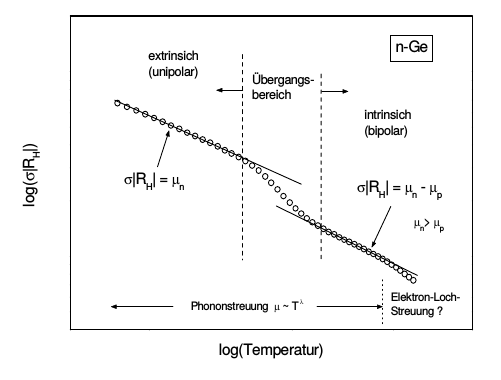
\includegraphics[scale=0.6]{./chap/Hallc_logTemp.png}
\caption{Hallkonstante über dem Logarithmus der Temperatur für n-dotiertes Germanium. Entnommen aus der Vorbereitungsmappe.}
\end{figure}

\subsubsection{Kontaktgeometrie}
In diesem Versuch werden zwei verschiedene Kontaktgeometrien verwendet.\\
Einerseits die herkömmliche Form eines Plättchens. Das ist Probe A aus Germanium. Wie aus der Schule bekannt wird ein Strom in x-Richtung und ein B-Feld in z-Richtung angelegt. Die Hallspannung kann dann senkrecht zu beiden, in y-Richtung abgegriffen werden. Die zu messenden Größen ergeben sich dann aus ihren Definitionen.
$$\sigma = \frac{J_x}{E_x}$$
$$\vert R_H \vert = \vert E_H/(J_x B_z) \vert$$

Die zweite Geometrie ist eine 4-Punktkontakt Messung nach Van-der-Pauw. Damit lassen sich obige Größen für einen Körper beliebiger Form bestimmen. \\
Angewendet wird das bei Probe B, einer Galliumarsenid-Probe mit 2D Elektronengas. In unserem Fall ist es eine symmetrische Form, wodurch sich zusammen mit dem 2D Elektronengas im Vergleich zur allgemeinen Form stark vereinfachte Gleichungen ergeben:
$$\sigma = \frac{\log 2}{\pi} \frac{I_{AB}}{U_{CD}} $$
$$R_H = \frac{\Delta U_{BD}}{I_{AC} \cdot B} $$

\newpage

\section{Versuchsaufbau}
Der Versuch wird an zwei Proben durchgeführt, oben erwähnte Proben A und B. Beide befinden sich elektrisch getrennt in dem selben Kryostaten und werden separat mit Strom versorgt bzw. vermessen. \\
Der Kryostat kühlt mit flüssigem Stickstoff, wobei die Kühlung über ein Gas-Auslassventil gesteuert werden kann. Auch bei hohen Temperaturen sollte die Kühlung zum Einstellen der Temperatur nicht abgeschaltet werden. Eine Heizwicklung heizt die Probe. Weiterhin wird ein Vakuum im Kryostaten mit einer Drehschiebepumpe erzeugt, um thermisch zu isolieren. \\
Die Temperatur wird über ein Proportional-Differential-Integral Regler (PID) eingestellt. Die jeweiligen Parameter müssen abhängig vom Temperaturbereich eingestellt werden. \\
Das angelegte B-Feld wird von einer Spule erzeugt und durch die Stromstärke geregelt. Das Gerät ist gegen zu hohe Induktionsspannungen geschützt, wodurch es schwer ist hier etwas falsch zu machen. \\
Für jede Probe gibt es außerdem eine Vorrichtung, um die Hallspannung oder die Leitspannung abzulesen. Diese beiden Werte werden verwendet, um die Leitfähigkeit, bzw. die Hallkonstante zu berechnen.

